\documentclass[10pt,letterpaper]{article}
% Course manuscript: single-column academic typography, 10-point body text.
\usepackage[textwidth=6in,textheight=9.15in,top=.9in,headheight=12pt,headsep=20pt,footskip=26pt]{geometry}
\usepackage[T1]{fontenc}
\usepackage{mathptmx,microtype,amsmath,amssymb}
\usepackage{graphicx,booktabs,tabularx,array,enumitem,xcolor}
\usepackage[authoryear,round]{natbib}
\usepackage[hidelinks]{hyperref}
\usepackage{xurl,caption,placeins}
\graphicspath{{output/figures/four_solvers/}}
\hypersetup{pdftitle={Classical Optimization Algorithms for Lasso Regression: A Four-Solver Comparison},pdfauthor={COMP6704 Group 9}}
\captionsetup{font=small,labelfont=bf,labelsep=period,skip=6pt}
\captionsetup[table]{position=top}
\setlength{\parindent}{0pt}\setlength{\parskip}{4pt}
\setlength{\emergencystretch}{2em}
\setlength{\textfloatsep}{10pt plus2pt minus2pt}
\setlength{\intextsep}{10pt plus2pt minus2pt}
\setlength{\floatsep}{9pt plus2pt minus2pt}
\renewcommand{\arraystretch}{1.08}
\renewcommand{\topfraction}{.92}\renewcommand{\bottomfraction}{.8}
\renewcommand{\textfraction}{.06}\renewcommand{\floatpagefraction}{.8}
\setcounter{topnumber}{3}\setcounter{bottomnumber}{2}\setcounter{totalnumber}{5}
\widowpenalty=10000\clubpenalty=10000\raggedbottom
\newcolumntype{Y}{>{\raggedright\arraybackslash}X}
\newcommand{\R}{\mathbb{R}}\newcommand{\soft}{\mathcal{S}}
\newcommand{\projectrepository}{\url{https://github.com/Caiyangxiao/COMP6704-Group9-Project}}
\begin{document}
\begin{center}
\hrule height4pt\vspace{.15in}
{\fontsize{17}{20}\selectfont\bfseries Classical Optimization Algorithms\\for Lasso Regression\par}
\vspace{5pt}{\large A Four-Solver Review and Empirical Comparison\par}
\vspace{.12in}\hrule height1pt\vspace{10pt}
{\bfseries COMP6704 Group Project --- Group 9\par}
{Convex Optimization\par}\vspace{9pt}
\begin{minipage}[t]{.48\linewidth}\centering\small
\textbf{CAI Yangxiao}\par Student ID: 26023041R\par
\href{mailto:26023041r@connect.polyu.hk}{26023041r@connect.polyu.hk}
\end{minipage}\hfill
\begin{minipage}[t]{.48\linewidth}\centering\small
\textbf{XUE Pengyu}\par Student ID: 26022951R\par
\href{mailto:26022951r@connect.polyu.hk}{26022951r@connect.polyu.hk}
\end{minipage}\par\vspace{7pt}
\begin{minipage}[t]{.48\linewidth}\centering\small
\textbf{ZHANG Kejia}\par Student ID: 26049131R\par
\href{mailto:26049131r@connect.polyu.hk}{26049131r@connect.polyu.hk}
\end{minipage}\hfill
\begin{minipage}[t]{.48\linewidth}\centering\small
\textbf{ZHOU Xiyu}\par Student ID: 26025265R\par
\href{mailto:26025265r@connect.polyu.hk}{26025265r@connect.polyu.hk}
\end{minipage}\par\vspace{5pt}
The Hong Kong Polytechnic University
\end{center}
\begin{abstract}
Lasso regression combines squared loss with an $\ell_1$ penalty to learn sparse linear models. We review its convex formulation and implement ISTA, standard FISTA, cyclic coordinate descent, and scaled ADMM. All four solve the same training problems and stop at a common proximal-gradient residual, with ADMM's factorization included in runtime. A fresh comparison uses three synthetic instances, one fixed Diabetes split, paired correlation and dimension studies, and ADMM penalty sensitivity. All 560 primary timing runs converge, with nearly identical final objectives and predictions. ISTA has the lowest mean time on independent-feature designs; ADMM is fastest on the recorded Diabetes split and has the lowest mean at the three positive correlation levels. Strongly correlated FISTA runs vary substantially. ADMM's setup cost grows with feature count, and its algorithmic penalty changes convergence speed without changing the Lasso estimator. Coefficient and regularization analyses distinguish numerical accuracy, sparse selection, and shrinkage error. Conclusions remain specific to the recorded implementations, datasets, and stopping rule.\footnote{Code and data repository: \projectrepository. Reproduction commands and saved evidence are described in Section~\ref{sec:reproducibility}.}
\end{abstract}

\section{Introduction and Literature Review}
Lasso adds an $\ell_1$ penalty to least-squares regression, shrinking coefficients and allowing exact zeros \citep{tibshirani1996}. A compact model can be easier to interpret when many predictors are available, while convexity makes global optimization tractable. Nonsmoothness at zero still leaves a meaningful algorithmic question: how should a solver exploit the loss, penalty, and predictor geometry to reach a prescribed accuracy?

This report asks three questions. First, how do full-vector thresholding, coordinate minimization, and splitting differ when the objective and stopping accuracy are fixed? Second, how do correlation and feature count change their measured efficiency? Third, how do the statistical penalty and ADMM's algorithmic penalty affect different parts of the problem? We contribute a reproducible implementation comparison, including controlled sensitivity studies, rather than a new optimization algorithm.

\subsection{Foundations and related solvers}
The literature links the four methods through a separable penalty and a quadratic loss. Iterative thresholding \citep{daubechies2004} and proximal algorithms \citep{parikh2014} explain ISTA; \mbox{\citet{beck2009}} establish FISTA's accelerated objective-error bound. Regression-specific coordinate updates appear in \citet{wu2008,friedman2010}, while \citet{tseng2001,wright2015} discuss convergence conditions and coordinate-selection rules. ADMM separates the two terms through an equality constraint and alternates a linear solve, thresholding, and a dual update \citep{boyd2011}.

Other work identifies costs outside a single update. LARS--Lasso constructs a solution path \citep{efron2004}; pathwise CD reuses nearby solutions \citep{friedman2010}. Interior-point methods use curvature and more involved linear algebra \citep{kim2007}. Adaptive restart changes momentum management \citep{odonoghue2015}, while Gap Safe screening removes variables certified inactive \citep{ndiaye2017}. These methods provide context but are not additional benchmarked implementations.

Statistical guarantees should also be separated from numerical ones. Coefficient agreement depends on uniqueness \citep{tibshirani2013}; correct support recovery requires assumptions on predictor relationships \citep{zhao2006}. An optimizer can accurately solve a Lasso problem whose selected variables or coefficient magnitudes differ from the generating model.

\subsection{Related regression penalties}
Ridge uses quadratic shrinkage to stabilize estimates under nonorthogonal predictors \citep{hoerl1970}. Elastic net combines sparsity with quadratic shrinkage and encourages grouped selection of correlated predictors \citep{zou2005}. Adaptive Lasso estimates penalty weights from an initial fit \citep{zou2006}; its objective remains convex after finite positive weights are fixed, with coordinate-specific thresholds. Table~\ref{tab:models} compares these estimators. Our experiments retain unweighted Lasso so that solver differences do not also change the model.
\begin{table}[!ht]\centering\small
\caption{Related convex penalties, paired with the same squared loss.}\label{tab:models}
\begin{tabularx}{\linewidth}{@{}l l Y@{}}\toprule
Model & Penalty & Main distinction\\\midrule
Ridge & $\alpha\|w\|_2^2/2$ & Usually dense coefficients\\
Lasso & $\lambda\|w\|_1$ & Exact zeros through uniform thresholds\\
Elastic net & $\lambda\|w\|_1+\alpha\|w\|_2^2/2$ & Sparsity and correlated-variable grouping\\
Adaptive Lasso & $\lambda\sum_j\omega_j|w_j|$ & Fixed weighted thresholds\\\bottomrule
\end{tabularx}\par\vspace{2pt}{\footnotesize $\alpha,\lambda>0$; fixed $\omega_j>0$.}
\end{table}

\section{Problem Formulation and Optimality}
\subsection{Training objective and preprocessing}
Let $X\in\R^{n\times d}$ contain training predictors, $y\in\R^n$ contain centered responses, and $w\in\R^d$ contain coefficients. Every solver minimizes
\begin{equation}
 F(w)=g(w)+h(w)=\frac{1}{2n}\|Xw-y\|_2^2+\lambda\|w\|_1,\qquad\lambda>0.
 \label{eq:objective}
\end{equation}
The factor $1/(2n)$ fixes the gradient and penalty scales. Training feature means and population standard deviations center and scale predictors; constant training columns are removed. Test data use those training statistics. Centering responses and restoring their training mean in predictions gives an unpenalized intercept without test leakage. Synthetic coefficient comparisons undo feature scaling to recover original units.

The constrained interpretation minimizes $g(w)$ subject to $\|w\|_1\leq t$. Any solution $w^\star$ of Eq.~\eqref{eq:objective} also solves that constrained problem for $t=\|w^\star\|_1$. For $t>0$, strict feasibility gives a multiplier $\lambda\geq0$; the correspondence need not be one-to-one \citep{boyd2004}. An exact convex quadratic-program formulation is
\begin{equation}
 \min_{w,v}\ \frac{\|Xw-y\|_2^2}{2n}+\lambda\mathbf{1}^\top v
 \quad\text{subject to}\quad -v\leq w\leq v.
 \label{eq:qp}
\end{equation}
Positive $\lambda$ forces $v_j=|w_j|$ at an optimum. The implemented solvers work directly with Eq.~\eqref{eq:objective}.

\subsection{Convexity, existence, and sparse optimality}
The gradient and Hessian of the loss are
\begin{equation}
 \nabla g(w)=X^\top(Xw-y)/n,\qquad \nabla^2g(w)=X^\top X/n\succeq0.
 \label{eq:gradient}
\end{equation}
The Hessian is positive semidefinite because $a^\top X^\top Xa=\|Xa\|_2^2\geq0$. Both terms in $F$ are convex. Since $F(w)\geq\lambda\|w\|_1$, it is coercive and has a minimizer. Full column rank of $X$ is sufficient for strong convexity and coefficient uniqueness, but is not necessary \citep{tibshirani2013}. If coefficients are nonunique, optimal fitted values still agree.

The KKT condition is necessary and sufficient for global optimality:
\begin{equation}
 0\in\nabla g(w^\star)+\lambda\partial\|w^\star\|_1.
 \label{eq:kkt}
\end{equation}
Thus $\nabla_jg(w^\star)=-\lambda\operatorname{sign}(w_j^\star)$ for nonzero coefficients, while $|\nabla_jg(w^\star)|\leq\lambda$ when $w_j^\star=0$. The interval $\partial|0|=[-1,1]$ permits exact zeros. The corner geometry of the $\ell_1$ ball gives the same intuition, but sparsity alone does not guarantee recovery of the true generating support.

\subsection{Soft thresholding and the penalty scale}
The separable proximal problem has a closed form \citep{parikh2014}:
\begin{equation}
 \operatorname*{arg\,min}_u\left\{\tfrac12\|u-v\|_2^2+\tau\|u\|_1\right\}
 =\soft_\tau(v),\quad
 \soft_\tau(v)_j=\operatorname{sign}(v_j)\max\{|v_j|-\tau,0\}.
 \label{eq:soft}
\end{equation}
When $X^\top X/n=I$, Eq.~\eqref{eq:objective} separates and $w^\star=\soft_\lambda(X^\top y/n)$. For example, $(1.2,-0.4,0.1)$ at threshold $0.3$ becomes $(0.9,-0.1,0)$. Retained coefficients shrink even when the active set is correct.

At zero, Eq.~\eqref{eq:kkt} gives the training-dependent reference penalty
\begin{equation}
 \lambda_{\max}=\|X^\top y/n\|_\infty.
 \label{eq:lmax}
\end{equation}
Zero is optimal for $\lambda\geq\lambda_{\max}$. The main comparison fixes $\lambda=0.1\lambda_{\max}$ to obtain nontrivial fits; it does not claim this value minimizes prediction error.

\section{Methodology: Four Optimization Algorithms}
\subsection{ISTA and standard FISTA}
The loss gradient is Lipschitz with $L=\|X\|_2^2/n$. For $0<\eta\leq1/L$, minimizing a quadratic upper bound on $g$ plus the exact penalty gives ISTA:
\begin{equation}
 w^{k+1}=\soft_{\eta\lambda}\bigl(w^k-\eta\nabla g(w^k)\bigr).
 \label{eq:ista}
\end{equation}
It combines a fitting step with thresholding and has a nonincreasing objective for the stated step size. The implementation uses matrix-vector products without a Gram matrix.

FISTA applies the same proximal step to an extrapolated point \citep{beck2009}. Initialize $z^1=w^0$, $t_1=1$, and set $\eta=1/L$:
\begin{align}
 w^k&=\soft_{\eta\lambda}\bigl(z^k-\eta\nabla g(z^k)\bigr),\\
 t_{k+1}&=(1+\sqrt{1+4t_k^2})/2,\\
 z^{k+1}&=w^k+\frac{t_k-1}{t_{k+1}}(w^k-w^{k-1}).
 \label{eq:fista}
\end{align}
Our implementation uses standard FISTA without restart or a monotonicity modification. For convex composite objectives with an existing minimizer and exact proximal steps, the objective-error bounds at step $1/L$ are
\begin{equation}
 F(w^k)-F^\star\leq
 \begin{cases}
 L\|w^0-w^\star\|_2^2/(2k),&\text{ISTA},\\
 2L\|w^0-w^\star\|_2^2/(k+1)^2,&\text{FISTA}.
 \end{cases}
 \label{eq:rates}
\end{equation}
These worst-case bounds concern objective error, not elapsed time, coefficient error, or the stopping residual. FISTA's objective and stationarity trajectory can oscillate.

\subsection{Cyclic coordinate descent}
CD fixes all coefficients except one and solves the scalar subproblem exactly. For column $x_j$, let $r^{(j)}=y-\sum_{\ell\ne j}x_\ell w_\ell$, using the latest coefficients. Then
\begin{equation}
 w_j\leftarrow\frac{\soft_\lambda(x_j^\top r^{(j)}/n)}{\|x_j\|_2^2/n}.
 \label{eq:cd}
\end{equation}
Maintaining $r=y-Xw$ gives $r^{(j)}=r+x_jw_j$ before the update and $r=r^{(j)}-x_jw_j$ afterwards. Each scalar update costs $O(n)$, and a complete sweep costs $O(nd)$ \citep{wu2008,friedman2010}. The denominator is one after training standardization, but the code retains the general formula.

Exact scalar minimization makes the objective nonincreasing. Convergence arguments use the separable nonsmooth penalty and additional regularity conditions \citep{tseng2001}; randomized-coordinate rates cannot be assigned directly to this cyclic implementation \citep{wright2015}.

\subsection{Scaled ADMM for the same Lasso objective}
ADMM introduces $x=z$ and minimizes $g(x)+\lambda\|z\|_1$ \citep{boyd2011}. We write its algorithmic penalty as $\beta>0$ to distinguish it from predictor correlation $\rho$ and model penalty $\lambda$. With scaled dual variable $u$, the augmented Lagrangian is
\begin{equation}
 \mathcal{L}_\beta(x,z,u)=g(x)+\lambda\|z\|_1
 +\frac{\beta}{2}\|x-z+u\|_2^2-\frac{\beta}{2}\|u\|_2^2.
\end{equation}
Alternating exact minimization and a dual update gives
\begin{align}
 (X^\top X/n+\beta I)x^{k+1}&=X^\top y/n+\beta(z^k-u^k),\label{eq:admmx}\\
 z^{k+1}&=\soft_{\lambda/\beta}(x^{k+1}+u^k),\\
 u^{k+1}&=u^k+x^{k+1}-z^{k+1}.\label{eq:admmu}
\end{align}
All three vectors start at zero. The normalized Gram matrix and right-hand side are formed once per solve; a cached Cholesky factor solves Eq.~\eqref{eq:admmx} without an explicit inverse. Positive $\beta$ makes the system positive definite even for rank-deficient $X$. The main comparison uses fixed $\beta=1$, without relaxation or adaptation.

The reported coefficient vector is $w=z$. Every objective value is therefore $F(z)$, with both terms evaluated at that vector. Evaluating the loss at $x$ and penalty at $z$ before feasibility would describe a different quantity. The common stopping residual is also evaluated at $z$. We additionally record primal residual $\|x-z\|_2$ and dual residual $\beta\|z^{k+1}-z^k\|_2$ as diagnostics.

Classical two-block ADMM convergence applies to closed proper convex terms with a saddle point, fixed positive penalty, and exact subproblem solves \citep{boyd2011}. Our finite-dimensional Lasso split has these properties. This asymptotic guarantee supplies no universal finite-time ordering against ISTA, FISTA, or CD.

\subsection{Complexity and fair comparison}
Table~\ref{tab:algorithms} distinguishes per-round work from preparation. Dense ADMM explicitly stores a $d\times d$ matrix; this implementation does not use sparse or Woodbury specializations. Its factorization is repeated inside every timed cold solve and is never reused across repetitions or instances. A CD sweep contains $d$ scalar updates, so fewer sweeps do not imply less computation than a vector or ADMM round.
\begin{table}[!ht]\centering\small
\caption{Implementation trade-offs for dense data. Monitoring is included in per-round work.}\label{tab:algorithms}
\begin{tabularx}{\linewidth}{@{}l l l Y@{}}\toprule
Method & Preparation & Per round & Distinctive cost / property\\\midrule
ISTA & $O(nd)$ & $O(nd)$ & Simple, monotone objective\\
FISTA & $O(nd)$ & $O(nd)$ & Extra momentum state; nonmonotone\\
Cyclic CD & $O(nd)$ & $O(nd)$ & Exact scalar solves in a Python loop\\
ADMM & $O(nd^2+d^3)$ & $O(nd+d^2)$ & Reusable factor within one solve; $O(d^2)$ extra storage\\\bottomrule
\end{tabularx}\par\vspace{2pt}{\footnotesize All methods store dense $X$; retaining $K$ history records adds $O(K)$ memory. The common spectral calculation is separate.}
\end{table}

\section{Experimental Design and Reproducibility}
\subsection{Data and paired sensitivity studies}
The main benchmark reads the four supplied CSVs, verifies their hashes, and retains their saved splits. Three synthetic instances use 300 observations, 50 independent standard-normal predictors, and 240/60 train/test rows. Only the first five generating coefficients are nonzero:
\[w_{\mathrm{true},1:5}=(2,-1.5,1,-2,1.5).\]
Gaussian noise has standard deviation $0.5$, and generation/split seeds are 0--2. Diabetes has 442 observations, ten baseline predictors, and a continuous measure of disease progression one year later \citep{efron2004,sklearn_data}; the saved split has 353/89 train/test rows. Its generating coefficients and true support are unknown.

The correlation study has 600 observations and 60 predictors in six blocks of ten. Independent standard-normal draws generate
\begin{equation}
 x_j=\sqrt{\rho}\,a_b+\sqrt{1-\rho}\,e_j,
 \qquad\rho\in\{0,0.5,0.9,0.99\}.
\end{equation}
Within each seed 10--12, correlation levels share underlying draws, noise, and a 480/120 split. Responses use the first five generating coefficients above. The dimension study fixes 1,000 observations and an 800/200 split while varying $d\in\{50,100,300,600\}$. Smaller matrices are prefixes of the same widest matrix and share its response within each seed.

CD also solves ratios $\lambda/\lambda_{\max}\in\{0.01,0.1,0.5,1\}$ on the four main inputs and 34 prespecified path values on synthetic seed 0 and Diabetes. These illustrate model sensitivity without test-based penalty selection. A separate ADMM study varies $\beta\in\{0.1,1,10\}$ on synthetic seed 0, Diabetes, and the three $\rho=0.99$ instances. It uses three timings per setting; the main benchmark remains at the predeclared $\beta=1$ regardless of these outcomes.

\subsection{Common accuracy and timing protocol}
For the same $L$ on each problem, define
\begin{align}
 G_L(w)&=L\left[w-\soft_{\lambda/L}\left(w-\nabla g(w)/L\right)\right],\\
 R(w)&=\frac{\|G_L(w)\|_\infty}{\max\{1,\|X^\top y/n\|_\infty\}}.
 \label{eq:residual}
\end{align}
The mapping is zero exactly at KKT stationarity. Each method checks $R\leq10^{-6}$ after a complete round, at the returned coefficients, with a 10,000-round cap. Small $R$ measures stationarity and is not an objective-error upper bound. ADMM's split residuals are additional diagnostics, not extra stopping conditions. Nonzeros satisfy $|w_j|>10^{-6}$ in standardized units.

All primary instance-method pairs have five timings, with method order rotated by repetition. We report each instance's median, then means and sample standard deviations across three synthetic or controlled instances. Diabetes remains one fixed split. Timing repetitions describe execution variation, not independent data uncertainty.

Elapsed time includes algorithm-specific preparation, factorization, objective/residual monitoring, and history recording. Loading, preprocessing, shared spectral-norm calculation, and plotting are excluded; spectral setup is saved separately. The preparation/iteration split refers to the representative median-time repetition. Thread limits are requested before imports and applied to detected numerical pools. All four algorithms are rerun on the same host; historical timings are retained separately and not pooled. The protocol was recorded in \texttt{experiment\_plan\_admm.md} before these measurements.

\subsection{Validation and reproduction}\label{sec:reproducibility}
Six numerical tests check the orthogonal solution for all methods, ADMM's normalized first update and returned vector, agreement with a tight scikit-learn reference across three $\beta$ values, the zero-solution threshold, an underdetermined rank-deficient design, and invalid algorithmic penalties. The experiment runner separately records analytic and reference checks. At validation tolerance $R\leq10^{-10}$, ADMM's largest orthogonal coefficient error was $1.16\times10^{-10}$; the other methods' errors were at most $1.11\times10^{-15}$. The largest relative objective difference from the tight nonorthogonal reference was $1.97\times10^{-12}$. These checks assess numerical correctness, not speed.

The rerun used Python 3.10.12, NumPy 2.2.6, SciPy 1.15.3, scikit-learn 1.7.2, and Matplotlib 3.10.9 on an x86\_64 Linux/WSL2 host. The two detected OpenBLAS pools and the OpenMP pool were limited to one thread. From \texttt{03\_Code\_and\_Results}, create an isolated Python environment and execute:
{\small
\begin{verbatim}
python -m pip install -r requirements-admm.txt
python -m unittest discover -s tests -v
python scripts/reproduce_four_solver_study.py --output results/reproduction-01
python scripts/plot_four_solver_results.py --results results/reproduction-01
python scripts/build_four_solver_report.py --results results/reproduction-01
\end{verbatim}
}
The first reproduction script runs the main, controlled, and ADMM sensitivity studies sequentially. The plot and report commands intentionally refresh the current figures and manuscript from the selected result root; keep their outputs together when compiling. The pinned rerun environment uses Python~3.10. The controlled generator retains the original paired design; new frozen inputs agree with historical arrays to $10^{-14}$, with only cross-platform floating-point rounding differences.
New directories preserve recorded results. Saved evidence includes all input hashes, actual controlled NPZ inputs, settings, runtime versions, code snapshots and checksums, coefficients, median-time histories, raw repetitions, and ADMM diagnostics. Python generates every new figure in PNG, SVG, and vector PDF; the report builder reads saved CSV/JSON values rather than rerunning fits. Exact runtimes vary by machine; numerical reproduction should first verify convergence and objective agreement.

\FloatBarrier
\section{Experimental Results and Analysis}
\subsection{Execution and fixed-penalty efficiency}
All 560 primary timing runs converged: 80 main and 480 controlled-study solves. All 16 four-ratio penalty fits, 68 path fits, and 45 ADMM sensitivity runs also converged. The largest within-problem relative objective spread in the controlled study was $8.61\times10^{-11}$. This numerical agreement supports the stated comparison accuracy without converting $R$ into an objective certificate.


\begin{table}[!htb]\centering\small
\caption{Four-solver comparison at $\lambda=0.1\lambda_{\max}$ and $R\leq10^{-6}$.}\label{tab:main}
\begin{tabular*}{\linewidth}{@{\extracolsep{\fill}}lrrrr@{}}\toprule
Method & Time (ms) & Rounds & Final $F$ & $R$ ($10^{-6}$)\\\midrule
\multicolumn{5}{l}{\textit{Synthetic: three instances}}\\
ISTA & $0.448 \pm 0.004$ & $24.7 \pm 0.6$ & $1.800 \pm 0.174$ & $0.71 \pm 0.16$\\
FISTA & $0.608 \pm 0.044$ & $30.7 \pm 2.3$ & $1.800 \pm 0.174$ & $0.53 \pm 0.30$\\
CD & $0.959 \pm 0.119$ & $5.0 \pm 0.0$ & $1.800 \pm 0.174$ & $0.14 \pm 0.17$\\
ADMM & $0.618 \pm 0.069$ & $24.0 \pm 1.0$ & $1.800 \pm 0.174$ & $0.89 \pm 0.09$\\
\midrule\multicolumn{5}{l}{\textit{Diabetes: one fixed split}}\\
ISTA & $1.510$ & 92 & $1812.178$ & $0.99$\\
FISTA & $1.449$ & 85 & $1812.178$ & $0.31$\\
CD & $0.677$ & 14 & $1812.178$ & $0.40$\\
ADMM & $0.582$ & 28 & $1812.178$ & $0.75$\\
\bottomrule\end{tabular*}
\par\vspace{2pt}{\footnotesize Synthetic entries: mean $\pm$ sample SD across three instances. Time per instance is the median of five runs. All preparation is included.}
\end{table}

ISTA has the smallest synthetic mean time, $0.448 \pm 0.004$ ms. FISTA and ADMM take $0.608 \pm 0.044$ and $0.618 \pm 0.069$ ms; their nearby means do not establish a robust distinction. CD uses only five sweeps but makes 50 sequential scalar updates per sweep. Vectorized NumPy kernels and Python coordinate loops have different overheads, which this study does not separately profile.

On Diabetes, ADMM takes 0.582 ms and 28 rounds, versus CD's 0.677 ms and 14 sweeps. Its ten-dimensional factorization is small, and native triangular solves avoid a Python coordinate loop. This implementation-level result changes the historical three-solver conclusion and is based entirely on the new same-host run.
\begin{figure}[!htb]\centering
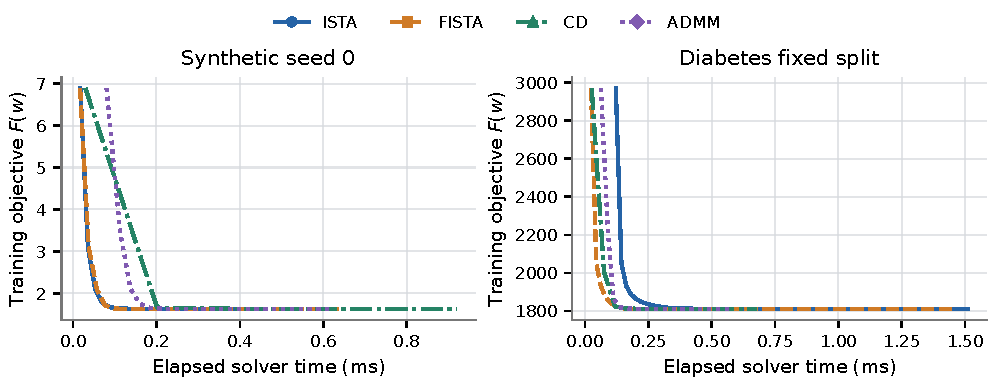
\includegraphics[width=\linewidth]{convergence.pdf}
\caption{Original Lasso objective versus elapsed time for representative median-time runs. ADMM includes factorization before its first update and evaluates $F(z)$ throughout.}\label{fig:objective}
\end{figure}
\begin{figure}[!htb]\centering
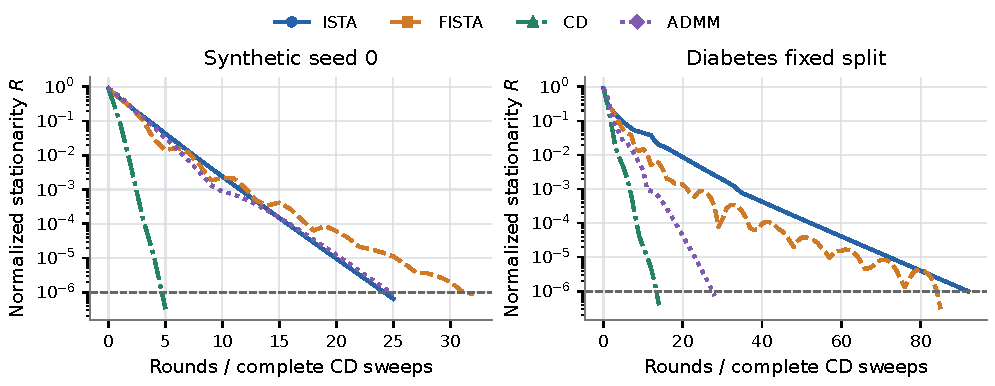
\includegraphics[width=\linewidth]{stationarity.pdf}
\caption{Common stationarity residual versus complete rounds. One CD round is a full coordinate sweep; one ADMM round contains all three split updates. Dashed line: $R=10^{-6}$.}\label{fig:stationarity}
\end{figure}

The objective and stationarity plots answer different questions. FISTA can reduce the objective early while its residual oscillates; its worst-case objective guarantee does not fix when this residual first crosses the threshold. ADMM's linear solve uses curvature information but incurs preparation and diagnostic costs. The comparison measures these implementations with monitoring, rather than isolated mathematical update costs.

\subsection{Timing variability and final solution quality}
Figure~\ref{fig:timing} retains all five main timings. Some synthetic timing ranges overlap because of occasional long repetitions, despite ISTA's lower medians. On Diabetes, ADMM's observed range (0.524--0.598 ms) lies below CD's (0.657--0.683 ms). ISTA and FISTA overlap. Neither five short repetitions nor three synthetic instances justify a general significance or population-level claim. Shared spectral setup, excluded from solver time, is reported in the raw environment records and would matter in an end-to-end deployment.
\begin{figure}[!htb]\centering
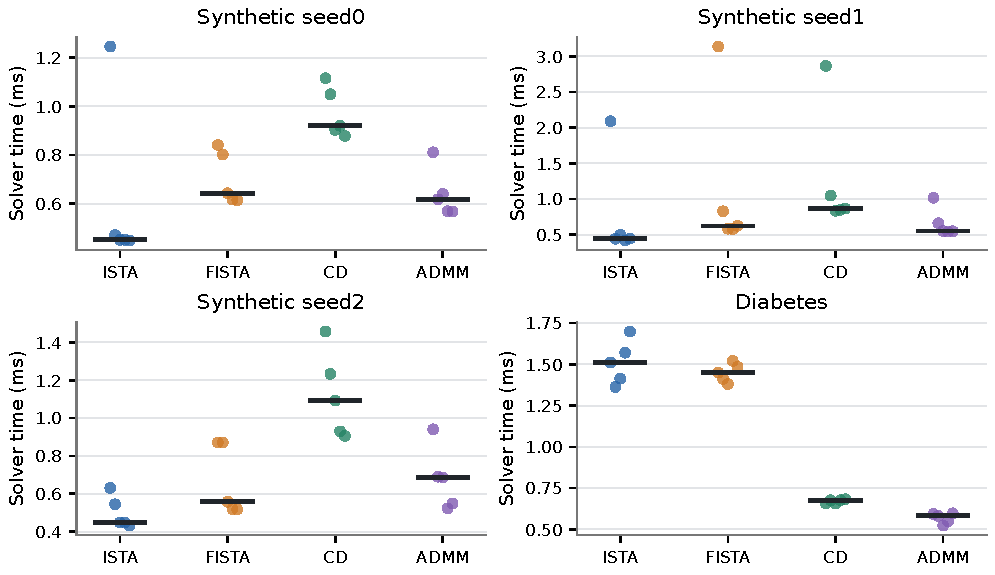
\includegraphics[width=\linewidth]{timing_repetitions.pdf}
\caption{All five main timings per instance and solver; black bars show medians. Repetitions quantify execution variation on fixed data.}\label{fig:timing}
\end{figure}

\begin{table}[!htb]\centering\small
\caption{Prediction and sparsity at the fixed penalty.}\label{tab:prediction}
\begin{tabular*}{\linewidth}{@{\extracolsep{\fill}}lrr@{}}\toprule
Method & Test MSE & Nonzero coefficients\\\midrule
\multicolumn{3}{l}{\textit{Synthetic: three instances}}\\
ISTA & $0.396 \pm 0.139$ & 5\\
FISTA & $0.396 \pm 0.139$ & 5\\
CD & $0.396 \pm 0.139$ & 5\\
ADMM & $0.396 \pm 0.139$ & 5\\
\midrule\multicolumn{3}{l}{\textit{Diabetes: one fixed split}}\\
ISTA & $2966.935$ & 5\\
FISTA & $2966.936$ & 5\\
CD & $2966.937$ & 5\\
ADMM & $2966.937$ & 5\\
\bottomrule\end{tabular*}
\par\vspace{2pt}{\footnotesize Synthetic: mean $\pm$ sample SD; nonzero means $|w_j|>10^{-6}$ in standardized units.}
\end{table}

All four methods retain five coefficients on every main instance. Diabetes test MSE differs by only 0.0017 on a scale near 2967; this does not establish predictive superiority of an optimizer. Similar predictions at one penalty are expected when accurate methods solve the same model. On synthetic data, the selected indices match the known generating support; on Diabetes, the same nonzero count cannot be interpreted as recovery accuracy.

\subsection{Sparse support, shrinkage, and model regularization}
The synthetic fits retain the five generating variables, yet their magnitudes shrink. Figure~\ref{fig:coefficients} uses CD as a representative converged solution and converts synthetic coefficients back to original units. The five active coefficient means are
\[(1.801,-1.260,0.736,-1.810,1.287),\]
with mean absolute active-coefficient error $0.221 \pm 0.025$. Exact support recovery therefore coexists with shrinkage error. The Diabetes fit retains sex, bmi, bp, s3, and s5. The Diabetes coefficients describe a standardized association on one split, not causal effects or stable selection across resampled data.
\begin{figure}[!htb]\centering
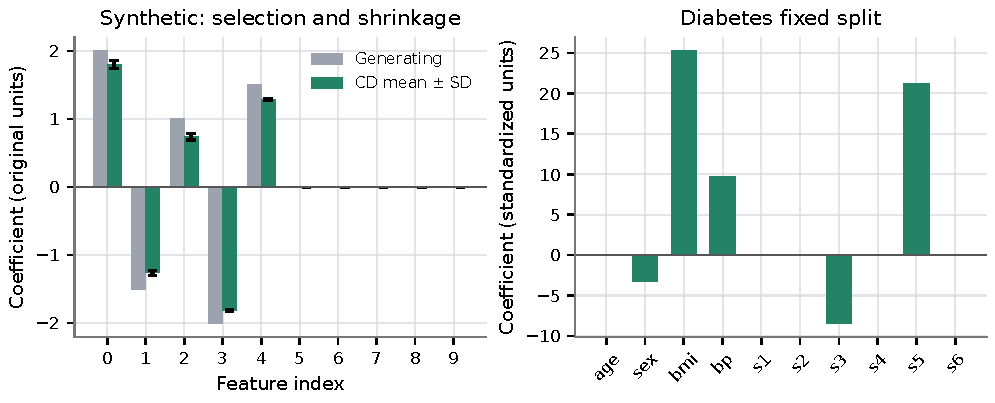
\includegraphics[width=\linewidth]{coefficient_analysis.pdf}
\caption{Representative CD coefficients at $0.1\lambda_{\max}$. Synthetic means and sample SD are compared with known coefficients in original units; Diabetes uses standardized units and has no known true support.}\label{fig:coefficients}
\end{figure}

\begin{table}[!htb]\centering\small
\caption{Model-penalty sensitivity using CD.}\label{tab:penalty}
\begin{tabular*}{\linewidth}{@{\extracolsep{\fill}}rrr@{}}\toprule
$\lambda/\lambda_{\max}$ & Test MSE & Nonzero coefficients\\\midrule
\multicolumn{3}{l}{\textit{Synthetic: three instances}}\\
0.01 & $0.236 \pm 0.033$ & $22.3 \pm 3.5$\\
0.1 & $0.396 \pm 0.139$ & $5.0 \pm 0.0$\\
0.5 & $5.506 \pm 1.021$ & $4.3 \pm 0.6$\\
1 & $11.945 \pm 1.311$ & $0.0 \pm 0.0$\\
\midrule\multicolumn{3}{l}{\textit{Diabetes: one fixed split}}\\
0.01 & $2912.647$ & $8.0$\\
0.1 & $2966.937$ & $5.0$\\
0.5 & $3837.820$ & $2.0$\\
1 & $5893.048$ & $0.0$\\
\bottomrule\end{tabular*}
\par\vspace{2pt}{\footnotesize Synthetic: mean $\pm$ sample SD over three instances. No penalty is selected using these test scores.}
\end{table}

Stronger regularization reduces selected variables in these cases while increasing average test error. On synthetic data, ratio 0.01 retains 22.3 variables on average and has MSE 0.236; ratio 0.1 retains the five generating variables but has MSE 0.396. The smaller model is more selective without attaining the lowest prediction error. Individual seed errors need not be monotone. At ratio 1, zero coefficients are optimal and predictions equal the training response mean. This behavior concerns the estimator, not the relative computation of the solvers.
\begin{figure}[!htb]\centering
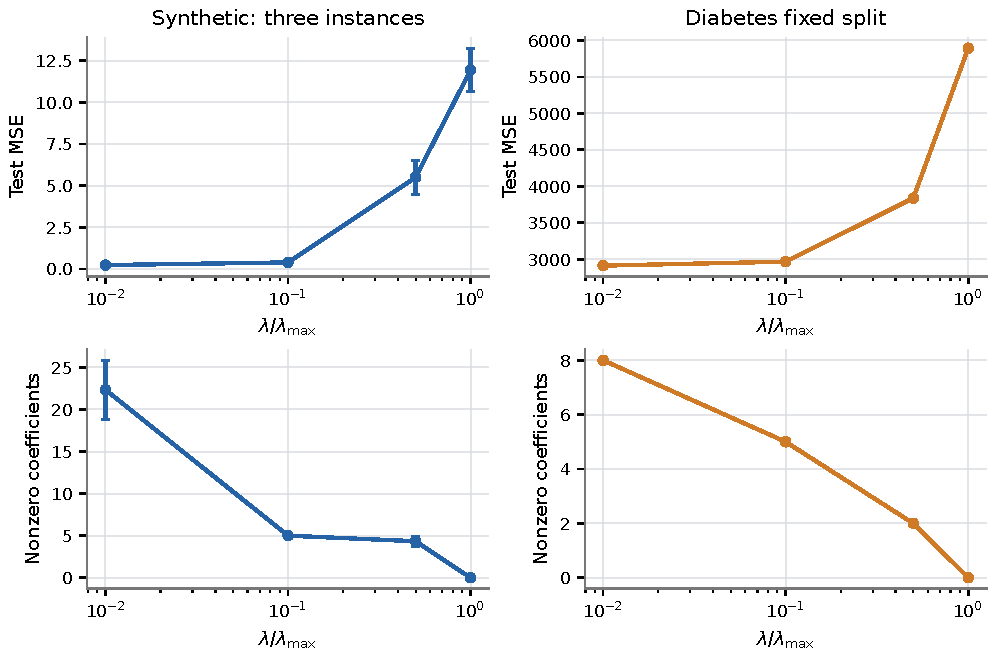
\includegraphics[width=\linewidth]{regularization.pdf}
\caption{CD penalty sensitivity: prediction error and nonzero counts on the saved splits. Synthetic panels summarize three instances. Test scores are descriptive and are not used to tune the penalty.}\label{fig:regularization}
\end{figure}
The saved 34-point coefficient paths provide a finer view of the same trade-off. Correlated predictors can redistribute a shared signal, so individual coefficient magnitudes need not change monotonically. Figure~\ref{fig:paths} shows the coefficient and error paths; the four-ratio table gives the across-instance summary.
\begin{figure}[!htb]\centering
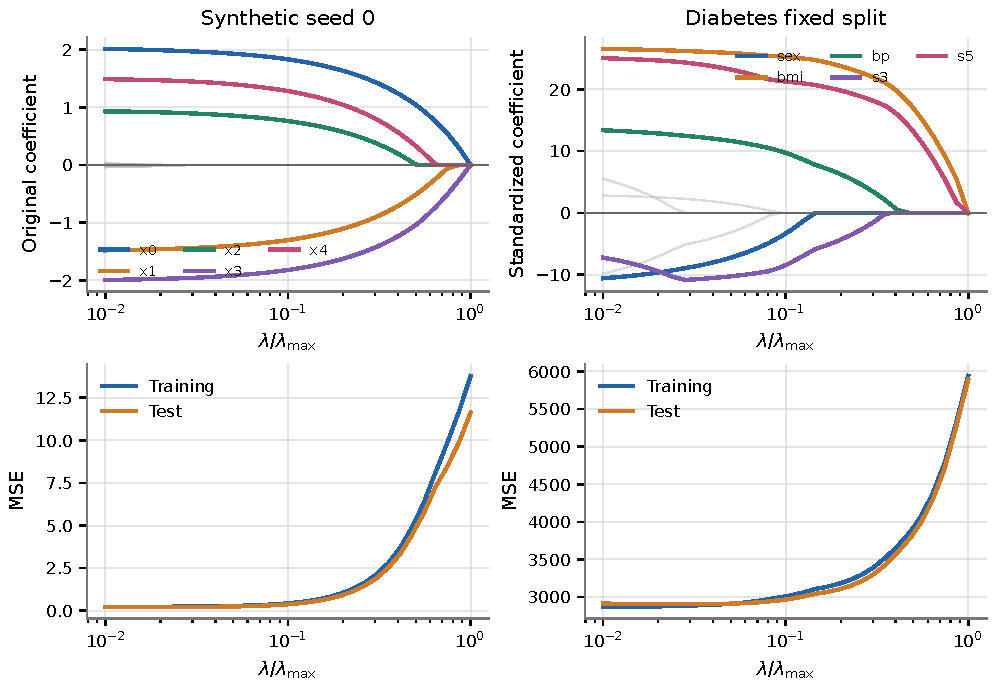
\includegraphics[width=\linewidth]{coefficient_paths.pdf}
\caption{CD coefficient paths and training/test MSE over 34 prespecified penalties. Colored synthetic paths are the true active variables; colored Diabetes paths are those selected at the main ratio 0.1, with no known true support. Gray paths are the remaining coefficients.}\label{fig:paths}
\end{figure}

\subsection{Correlation changes the computational ranking}\label{sec:correlation}

\begin{table}[!htb]\centering\small
\caption{Correlation sensitivity: full-Gram condition number and time (ms).}\label{tab:correlation}
\begin{tabular*}{\linewidth}{@{\extracolsep{\fill}}rrrrrr@{}}\toprule
$\rho$ & $\kappa$ & ISTA & FISTA & CD & ADMM\\\midrule
0 & 4.1 & $0.525\pm0.134$ & $0.670\pm0.011$ & $1.273\pm0.064$ & $0.736\pm0.089$\\
0.5 & 28.8 & $3.937\pm0.486$ & $4.517\pm0.495$ & $5.193\pm0.470$ & $1.326\pm0.077$\\
0.9 & 230.3 & $28.369\pm3.512$ & $21.505\pm3.074$ & $27.031\pm1.810$ & $3.114\pm0.163$\\
0.99 & 2492.8 & $177.997\pm16.772$ & $24.041\pm23.123$ & $101.630\pm18.160$ & $17.457\pm1.401$\\
\bottomrule\end{tabular*}
\par\vspace{2pt}{\footnotesize Time: mean $\pm$ sample SD of three instance medians, each from five runs.}
\end{table}

At $\rho=0$, ISTA has the lowest mean time. ADMM has the lowest mean at $\rho=0.5$, $0.9$, and $0.99$. At $\rho=0.99$, ADMM takes $17.457\pm1.401$ ms, compared with FISTA's $24.041\pm23.123$ ms. However, FISTA is faster on 2 of the three instances; one slower FISTA instance raises its mean. The average therefore supports a conditional comparison, not uniform ADMM dominance. Acceleration still sharply improves on ISTA in the highly correlated setting.
The full-Gram condition number rises from 4.1 to 2492.8, exposing weak-curvature directions. It is a diagnostic rather than a complete runtime predictor: support, penalty scale, monitoring, and the update mechanism also matter. ADMM factors a regularized Gram matrix; FISTA uses the same fixed gradient step as ISTA with extrapolation. Different uses of curvature help explain why the independent-feature ranking need not persist.
\begin{figure}[!htb]\centering
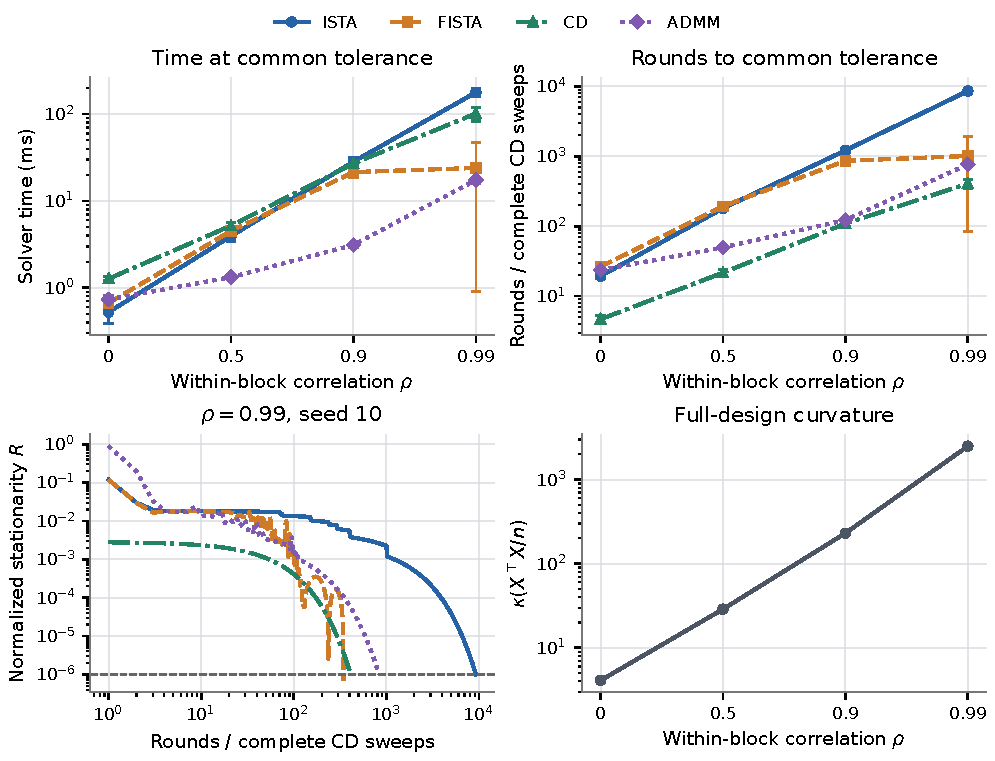
\includegraphics[width=\linewidth]{correlation_comparison.pdf}
\caption{Paired correlation study: solver time, rounds, seed-10 residual at $\rho=0.99$, and full-design condition number. Error bars are sample SD across three instance medians, each based on five timings.}\label{fig:correlation}
\end{figure}

\subsection{Feature count and the cost of factorization}
ISTA has the smallest mean time at every tested feature count. Its rounds rise from 15.0 at $d=50$ to 43.3 at $d=600$. CD needs four sweeps throughout, yet each sweep becomes more expensive as it visits more coordinates. At $d=600$, ISTA takes 10.582 ms, CD 12.332 ms, FISTA 13.499 ms, and ADMM 17.413 ms. ADMM uses fewer rounds than ISTA at this width but pays for Gram construction, factorization, and triangular solves. The measured preparation breakdown in Table~\ref{tab:setup} exposes that cost rather than attributing runtime to round count alone.
\begin{figure}[!htb]\centering
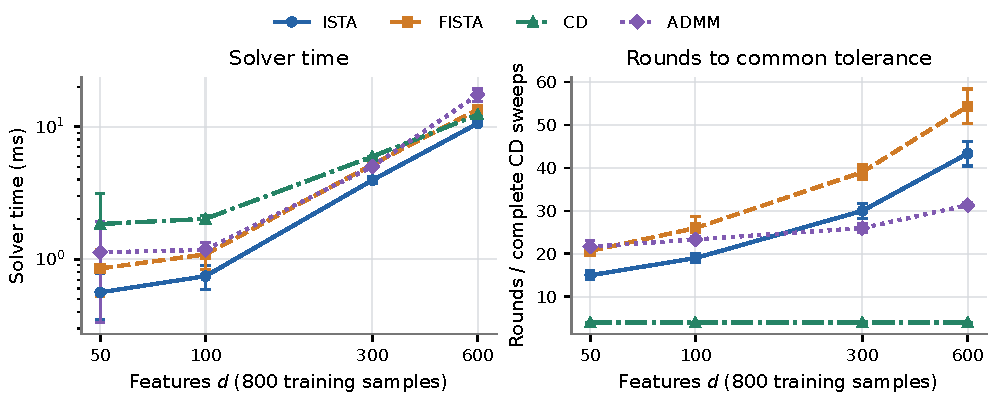
\includegraphics[width=\linewidth]{dimension_comparison.pdf}
\caption{Paired feature-count study with 800 training observations. Means and sample SD across three instance medians. ADMM's cold setup is included; CD rounds are complete sweeps.}\label{fig:dimension}
\end{figure}

\begin{table}[!htb]\centering\small
\caption{ADMM preparation within cold total time in the dimension study.}\label{tab:setup}
\begin{tabular*}{\linewidth}{@{\extracolsep{\fill}}rrrr@{}}\toprule
$d$ & Total (ms) & Preparation (ms) & Preparation / total\\\midrule
50 & $1.126$ & $0.175$ & $15.5\%$\\
100 & $1.178$ & $0.317$ & $26.9\%$\\
300 & $5.013$ & $1.908$ & $38.1\%$\\
600 & $17.413$ & $8.251$ & $47.4\%$\\
\bottomrule\end{tabular*}
\par\vspace{2pt}{\footnotesize Means across three representative median-time runs. Last column is the ratio of the displayed means; preparation includes the first common check.}
\end{table}

Preparation can be amortized in other workloads, but no factorization is shared here. A warm-started regularization path, compiled CD, sparse data, or a Woodbury ADMM implementation would be a distinct benchmark rather than an explanation established by these timings.

\subsection{ADMM penalty sensitivity}

\begin{table}[!htb]\centering\small
\caption{ADMM algorithmic-penalty sensitivity at fixed model penalty.}\label{tab:sensitivity}
\begin{tabular*}{\linewidth}{@{\extracolsep{\fill}}lrrr@{}}\toprule
Input & $\beta$ & Time (ms) & ADMM rounds\\\midrule
Synthetic seed 0 & 0.1 & $2.980$ & $142.0$\\
 & 1 & $0.600$ & $25.0$\\
 & 10 & $3.342$ & $157.0$\\
Diabetes & 0.1 & $3.849$ & $193.0$\\
 & 1 & $0.560$ & $28.0$\\
 & 10 & $4.598$ & $249.0$\\
Correlation 0.99 & 0.1 & $15.493 \pm 2.991$ & $656.0 \pm 174.0$\\
 & 1 & $18.713 \pm 1.308$ & $769.3 \pm 55.4$\\
 & 10 & $182.095 \pm 17.006$ & $7655.0 \pm 556.8$\\
\bottomrule\end{tabular*}
\par\vspace{2pt}{\footnotesize Three timings per setting; correlation entries summarize three instance medians. These runs are separate from the five-repeat main comparison.}
\end{table}

Among the three tested settings, $\beta=1$ has the smallest time and round count on synthetic seed 0 and Diabetes. The highly correlated three-instance mean is lower at $\beta=0.1$ than at $1$, but this is not true on every seed. At $\beta=10$, the highly correlated fits need roughly 7,200--8,300 rounds and are much slower, although all meet the same accuracy threshold. Thus a fixed default is not uniformly optimal. The sensitivity outcomes do not retroactively tune the main comparison, and runtime changes do not establish changes in predictive quality.
\begin{figure}[!htb]\centering
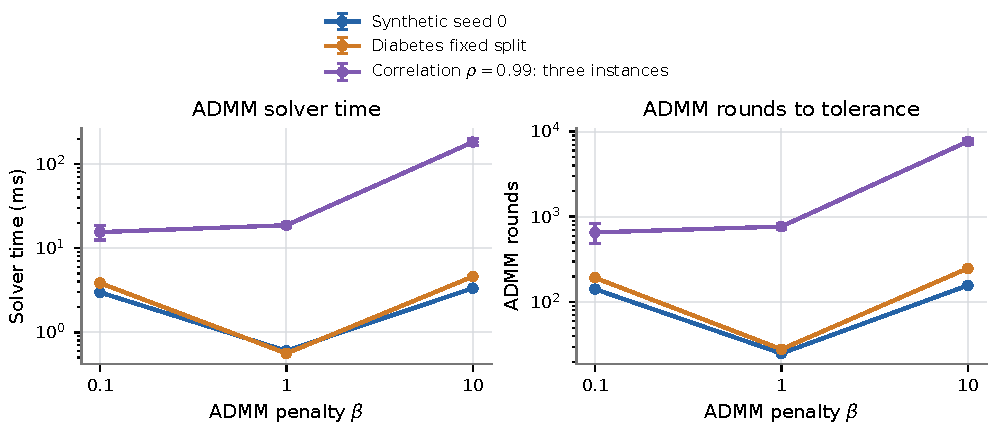
\includegraphics[width=\linewidth]{admm_penalty_sensitivity.pdf}
\caption{ADMM algorithmic-penalty sensitivity at fixed Lasso $\lambda$ and stopping tolerance. Main inputs have one fixed instance each; the highly correlated summary uses three instance medians. Each setting has three timing repetitions.}\label{fig:admm_sensitivity}
\end{figure}
The primal and dual residuals need not fall at the same rate. Their saved traces help diagnose the split iteration, while the common $R(z)$ determines accuracy for every solver. Changing $\beta$ changes the algorithm; changing $\lambda$ changes the estimator. Keeping those roles separate prevents a parameter-tuning advantage from being mistaken for a different predictive model.

\FloatBarrier
\section{Limitations and Conclusions}
The study covers small dense designs, four block-correlation levels, and feature counts up to 600. It does not benchmark underdetermined or sparse problems, compiled coordinate loops, adaptive ADMM penalties, restarted FISTA, or screening. One correctness test uses a rank-deficient design, but it is not a runtime study. Python loops, native linear-algebra kernels, and monitoring costs influence the measured ordering. A single Diabetes split cannot establish selection stability, and three synthetic instances provide limited descriptive variation.

The shared residual gives a consistent stopping rule, not a bound on objective error. ADMM setup is included while the shared spectral calculation is excluded; other cost conventions may change end-to-end conclusions. No penalty was selected by test error, and no confidence interval or significance claim is inferred from the small timing samples.

The four methods reach nearly identical Lasso solutions while exposing distinct computational trade-offs. ISTA is fastest on the tested independent-feature designs. ADMM is fastest on the saved Diabetes split and has the smallest mean at positive block correlations, while FISTA wins on two of the three most-correlated instances. ADMM's dense preparation becomes material as feature count grows, and its algorithmic penalty changes convergence speed. The statistical penalty instead changes sparsity and shrinkage, often trading a smaller model for higher test error. Future comparisons should examine compiled CD, adaptive or structure-aware ADMM, restarted FISTA, dual-gap certificates, and validation-selected penalties over repeated real-data splits.

\subsection*{Author contributions}
All four members contributed to report writing and revision, experimental design, and experimental evaluation. The individual implementation and presentation responsibilities are listed below.
\begin{center}\small
\begin{tabularx}{\linewidth}{@{}l l Y@{}}\toprule
Member (student ID) & Algorithm implementation & Presentation and slide responsibilities\\\midrule
\shortstack[l]{CAI Yangxiao\\26023041R} & ADMM & Part I\\[3pt]
\shortstack[l]{XUE Pengyu\\26022951R} & FISTA & Part II\\[3pt]
\shortstack[l]{ZHANG Kejia\\26049131R} & Cyclic CD & Introduction and work overview; PPT design\\[3pt]
\shortstack[l]{ZHOU Xiyu\\26025265R} & ISTA & Part III\\\bottomrule
\end{tabularx}
\end{center}

\subsection*{Generative AI assistance}
Generative AI tools assisted with literature organization, implementation, drafting, and language and formatting revision. The four-solver measurements were executed locally and retained with configurations, inputs, code snapshots, and validation outputs.

\begingroup\small
\begin{thebibliography}{}
\setlength{\itemsep}{1pt}\setlength{\parskip}{0pt}
\bibitem[Beck and Teboulle(2009)]{beck2009}
Amir Beck and Marc Teboulle. 2009.
\href{https://doi.org/10.1137/080716542}{A fast iterative shrinkage-thresholding algorithm for linear inverse problems}.
\emph{SIAM Journal on Imaging Sciences}, 2(1):183--202.

\bibitem[Boyd and Vandenberghe(2004)]{boyd2004}
Stephen Boyd and Lieven Vandenberghe. 2004.
\href{https://web.stanford.edu/~boyd/cvxbook/}{Convex Optimization}.
Cambridge University Press.

\bibitem[Boyd et~al.(2011)Boyd, Parikh, Chu, Peleato, and Eckstein]{boyd2011}
Stephen Boyd, Neal Parikh, Eric Chu, Borja Peleato, and Jonathan Eckstein. 2011.
\href{https://doi.org/10.1561/2200000016}{Distributed optimization and statistical learning via the alternating direction method of multipliers}.
\emph{Foundations and Trends in Machine Learning}, 3(1):1--122.

\bibitem[Daubechies et~al.(2004)Daubechies, Defrise, and De~Mol]{daubechies2004}
Ingrid Daubechies, Michel Defrise, and Christine De Mol. 2004.
\href{https://doi.org/10.1002/cpa.20042}{An iterative thresholding algorithm for linear inverse problems with a sparsity constraint}.
\emph{Communications on Pure and Applied Mathematics}, 57(11):1413--1457.

\bibitem[Efron et~al.(2004)Efron, Hastie, Johnstone, and Tibshirani]{efron2004}
Bradley Efron, Trevor Hastie, Iain Johnstone, and Robert Tibshirani. 2004.
\href{https://doi.org/10.1214/009053604000000067}{Least angle regression}.
\emph{The Annals of Statistics}, 32(2):407--451.

\bibitem[Friedman et~al.(2010)Friedman, Hastie, and Tibshirani]{friedman2010}
Jerome H. Friedman, Trevor Hastie, and Rob Tibshirani. 2010.
\href{https://doi.org/10.18637/jss.v033.i01}{Regularization paths for generalized linear models via coordinate descent}.
\emph{Journal of Statistical Software}, 33(1):1--22.

\bibitem[Hoerl and Kennard(1970)]{hoerl1970}
Arthur E. Hoerl and Robert W. Kennard. 1970.
\href{https://doi.org/10.1080/00401706.1970.10488634}{Ridge regression: Biased estimation for nonorthogonal problems}.
\emph{Technometrics}, 12(1):55--67.

\bibitem[Kim et~al.(2007)Kim, Koh, Lustig, Boyd, and Gorinevsky]{kim2007}
Seung-Jean Kim, Kwangmoo Koh, Michael Lustig, Stephen Boyd, and Dimitry Gorinevsky. 2007.
\href{https://doi.org/10.1109/JSTSP.2007.910971}{An interior-point method for large-scale $\ell_1$-regularized least squares}.
\emph{IEEE Journal on Selected Topics in Signal Processing}, 1(4):606--617.

\bibitem[Ndiaye et~al.(2017)Ndiaye, Fercoq, Gramfort, and Salmon]{ndiaye2017}
Eugene Ndiaye, Olivier Fercoq, Alexandre Gramfort, and Joseph Salmon. 2017.
\href{https://jmlr.org/papers/v18/16-577.html}{Gap Safe screening rules for sparsity enforcing penalties}.
\emph{Journal of Machine Learning Research}, 18(128):1--33.

\bibitem[O'Donoghue and Cand\`es(2015)]{odonoghue2015}
Brendan O'Donoghue and Emmanuel Cand\`es. 2015.
\href{https://doi.org/10.1007/s10208-013-9150-3}{Adaptive restart for accelerated gradient schemes}.
\emph{Foundations of Computational Mathematics}, 15:715--732.

\bibitem[Parikh and Boyd(2014)]{parikh2014}
Neal Parikh and Stephen Boyd. 2014.
\href{https://doi.org/10.1561/2400000003}{Proximal algorithms}.
\emph{Foundations and Trends in Optimization}, 1(3):127--239.

\bibitem[scikit-learn developers(2026)]{sklearn_data}
scikit-learn developers.
\href{https://scikit-learn.org/stable/modules/generated/sklearn.datasets.load_diabetes.html}{Diabetes dataset}
and \href{https://scikit-learn.org/stable/modules/generated/sklearn.linear_model.Lasso.html}{Lasso}.
Online documentation; rerun software version: 1.7.2.

\bibitem[Tibshirani(1996)]{tibshirani1996}
Robert Tibshirani. 1996.
\href{https://doi.org/10.1111/j.2517-6161.1996.tb02080.x}{Regression shrinkage and selection via the lasso}.
\emph{Journal of the Royal Statistical Society: Series B (Methodological)}, 58(1):267--288.

\bibitem[Tibshirani(2013)]{tibshirani2013}
Ryan J. Tibshirani. 2013.
\href{https://doi.org/10.1214/13-EJS815}{The lasso problem and uniqueness}.
\emph{Electronic Journal of Statistics}, 7:1456--1490.

\bibitem[Tseng(2001)]{tseng2001}
Paul Tseng. 2001.
\href{https://doi.org/10.1023/A:1017501703105}{Convergence of a block coordinate descent method for nondifferentiable minimization}.
\emph{Journal of Optimization Theory and Applications}, 109(3):475--494.

\bibitem[Wright(2015)]{wright2015}
Stephen J. Wright. 2015.
\href{https://doi.org/10.1007/s10107-015-0892-3}{Coordinate descent algorithms}.
\emph{Mathematical Programming}, 151(1):3--34.

\bibitem[Wu and Lange(2008)]{wu2008}
Tong Tong Wu and Kenneth Lange. 2008.
\href{https://doi.org/10.1214/07-AOAS147}{Coordinate descent algorithms for lasso penalized regression}.
\emph{The Annals of Applied Statistics}, 2(1):224--244.

\bibitem[Zhao and Yu(2006)]{zhao2006}
Peng Zhao and Bin Yu. 2006.
\href{https://jmlr.org/papers/v7/zhao06a.html}{On model selection consistency of Lasso}.
\emph{Journal of Machine Learning Research}, 7(90):2541--2563.

\bibitem[Zou(2006)]{zou2006}
Hui Zou. 2006.
\href{https://doi.org/10.1198/016214506000000735}{The adaptive lasso and its oracle properties}.
\emph{Journal of the American Statistical Association}, 101(476):1418--1429.

\bibitem[Zou and Hastie(2005)]{zou2005}
Hui Zou and Trevor Hastie. 2005.
\href{https://doi.org/10.1111/j.1467-9868.2005.00503.x}{Regularization and variable selection via the elastic net}.
\emph{Journal of the Royal Statistical Society: Series B (Statistical Methodology)}, 67(2):301--320.

\end{thebibliography}
\endgroup

\end{document}
